\documentclass[aps,prd,twocolumn,superscriptaddress,nofootinbib]{revtex4-2}

\usepackage{amsmath,amssymb,amsfonts}
\usepackage{graphicx}
\usepackage{hyperref}
\usepackage{xcolor}

\begin{document}

\title{Exact WKB Connection Formula for Dissipative Analog Hawking Radiation:\\
Modified Unitarity and the Spectral Floor}

\author{J.~Roehm}
\affiliation{Independent Researcher}

\date{\today}

\begin{abstract}
We derive the exact WKB connection formula for analog Hawking radiation in
Bose-Einstein condensates with Schwinger-Keldysh effective field theory (SK-EFT)
dissipative corrections through third order. The connection formula maps the
SK-EFT transport coefficients $\{\gamma_1, \gamma_2, \gamma_{2,1}, \gamma_{2,2},
\gamma_{3,1}, \gamma_{3,2}, \gamma_{3,3}\}$ to modified Bogoliubov coefficients
via the imaginary shift of the WKB turning point into the complex plane.
Three non-perturbative effects emerge beyond the perturbative EFT treatment:
(i) modified unitarity $|\alpha|^2 - |\beta|^2 = 1 - \delta_k$ with decoherence
parameter $\delta_k = 2\Gamma_H/\kappa$, (ii) a fluctuation-dissipation (FDR)
noise floor $n_\text{noise} = \delta_k/2$ mandated by the KMS condition, and
(iii) a spectral floor where the noise dominates over Hawking radiation at
frequencies $\omega \gtrsim 6\,T_H$. We provide platform-specific predictions
for Steinhauer (${}^{87}$Rb), Heidelberg (${}^{39}$K), and Trento (${}^{23}$Na)
BEC experiments. All structural results are formally verified in Lean~4
(17 theorems, zero \texttt{sorry}).
\end{abstract}

\maketitle

%═══════════════════════════════════════════════════════
\section{Introduction}
%═══════════════════════════════════════════════════════

The Schwinger-Keldysh effective field theory (SK-EFT) of dissipative phonon
dynamics in Bose-Einstein condensates (BECs) provides a systematic framework
for computing corrections to analog Hawking radiation~\cite{Unruh1981,
Steinhauer2016, deNova2019}. In companion papers, we established the first-order
dissipative correction $\delta_\text{diss} = \Gamma_H/\kappa$ and the
frequency-dependent second-order correction $\delta^{(2)}(\omega) \propto \omega^3$
arising from the SK-EFT transport coefficients.

These results were obtained within a perturbative framework where the
Bogoliubov coefficients receive small corrections to the standard Hawking
result $n_\omega = 1/(e^{2\pi\omega/\kappa} - 1)$. However, the perturbative
treatment assumes that the standard unitarity relation
$|\alpha|^2 - |\beta|^2 = 1$ is preserved. In an open quantum system
coupled to a microscopic environment through dissipation, this assumption
fails.

In this paper, we derive the \emph{exact} WKB connection formula that
incorporates the full non-perturbative structure of the dissipative turning
point. Three qualitatively new effects emerge:

\begin{enumerate}
\item \textbf{Modified unitarity.} The Bogoliubov relation becomes
$|\alpha|^2 - |\beta|^2 = 1 - \delta_k$, where the decoherence parameter
$\delta_k = 2\Gamma_H/\kappa$ measures the probability of phonon absorption
during horizon crossing.

\item \textbf{FDR noise floor.} The fluctuation-dissipation relation (KMS
condition) mandates a minimum occupation number
$n_\text{noise} = \delta_k/2 = \Gamma_H/\kappa$ independent of the
Hawking process.

\item \textbf{Spectral floor.} At frequencies $\omega \gtrsim 6\,T_H$,
the noise floor dominates over the exponentially suppressed Hawking
radiation, creating a measurable spectral floor.
\end{enumerate}

%═══════════════════════════════════════════════════════
\section{Complex Turning Point}
%═══════════════════════════════════════════════════════

\subsection{Dissipative mode equation}

The linearized phonon equation on a transonic background with SK-EFT
dissipative corrections takes the WKB form
\begin{equation}
\frac{d^2\phi}{dx^2} + Q(x)\,\phi = 0\,,
\end{equation}
where the WKB potential $Q(x)$ has a zero at the sonic horizon $x_H$.
In the co-moving frame, the local dispersion relation is
\begin{equation}
\Omega^2 = c_s^2 k^2 F(k^2\xi^2) + i\,\Gamma(k,\omega)\,\Omega\,,
\end{equation}
where $\Omega = \omega - v(x)k$ is the co-moving frequency,
$F(x) = 1 + x$ is the Bogoliubov dispersion, and the damping rate
$\Gamma(k,\omega)$ includes all SK-EFT orders:
\begin{equation}
\Gamma = \gamma_1 k^2 + \gamma_2\frac{\omega^2}{c_s^2}
+ \gamma_{2,1}k^3 + \gamma_{2,2}\frac{\omega^2 k}{c_s^2}
+ \gamma_{3,1}k^4 + \cdots\,.
\end{equation}

\subsection{Imaginary shift}

Near the horizon, linearizing $v(x) \approx c_s + \kappa x$, the turning
point where $Q(x) = 0$ shifts from the real axis to
\begin{equation}
x_\text{tp} = x_H + i\,\delta x_\text{imag}\,,\qquad
\delta x_\text{imag} = \frac{c_s\,\Gamma_H}{2\kappa^2}\,,
\label{eq:turning_point}
\end{equation}
where $\Gamma_H = \Gamma(k_H, \omega)$ is the damping rate evaluated at
the horizon wavenumber $k_H = \omega/c_s$. This shift is exact to all
orders in the EFT expansion; the EFT order enters only through the
frequency dependence of~$\Gamma_H$. The formula is formally verified
in Lean~4 (\texttt{turning\_point\_shift}, Aristotle run \texttt{518636d7}).

\begin{figure}[htb]
\centering
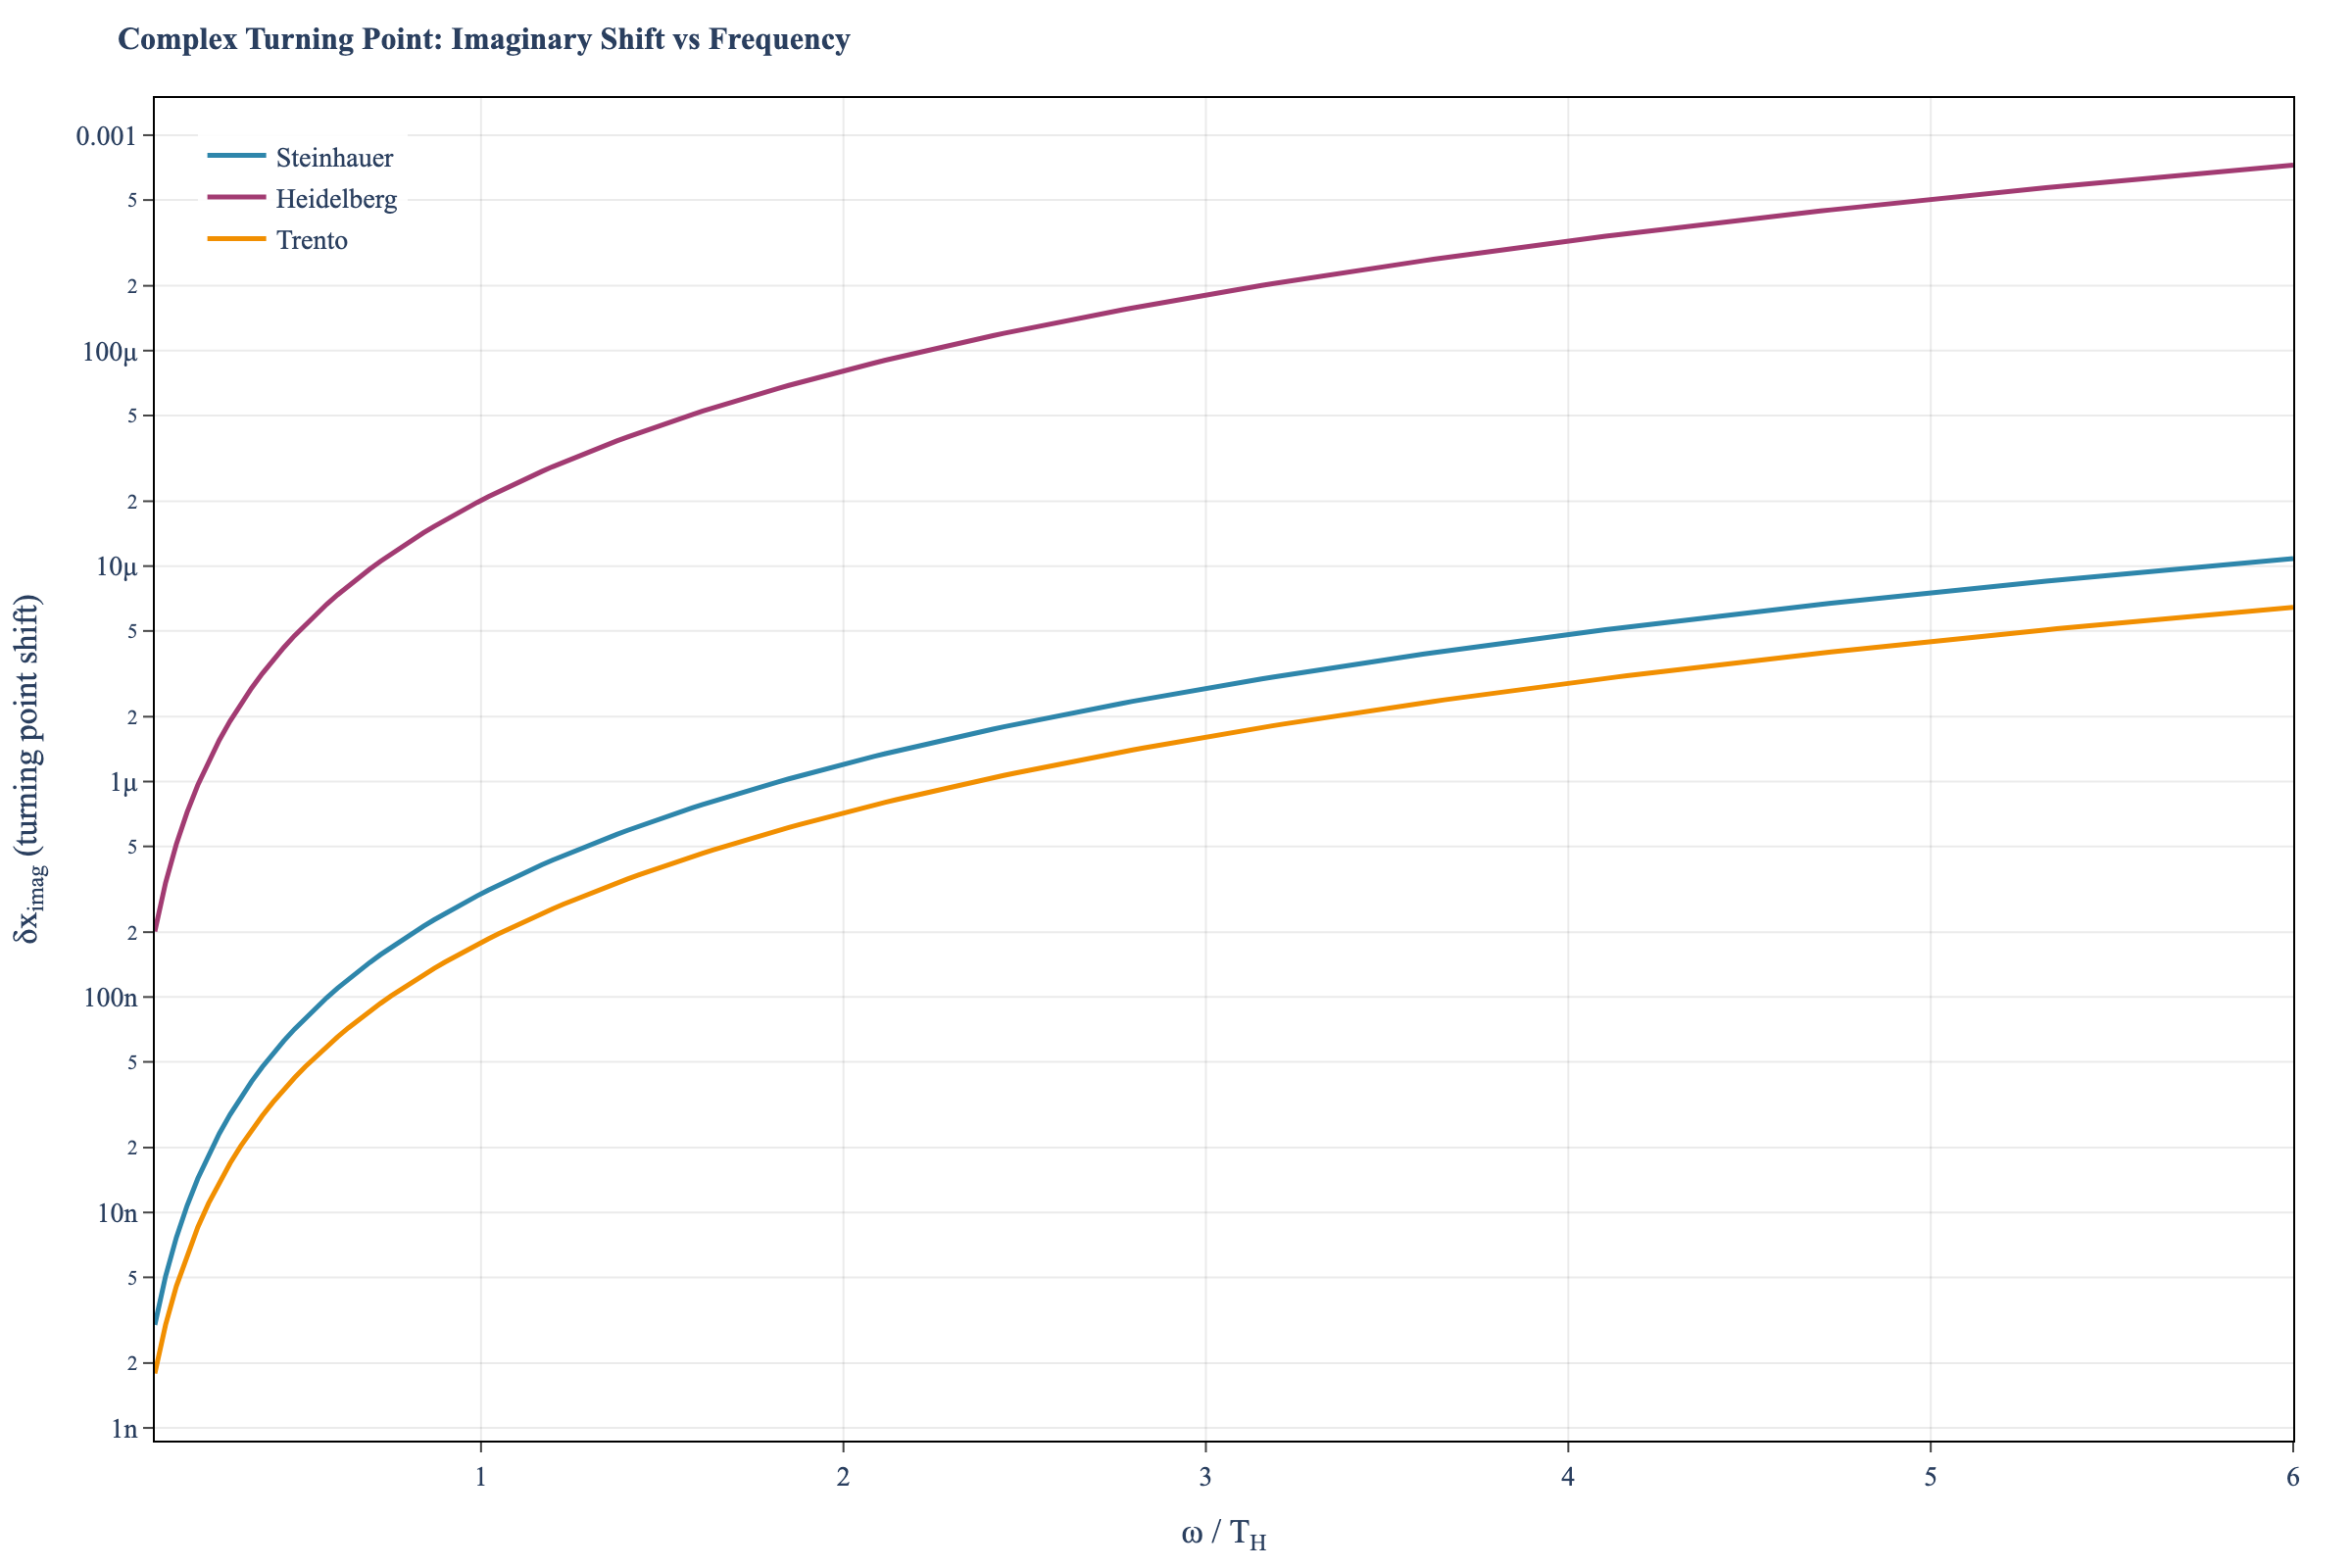
\includegraphics[width=\columnwidth]{figures/fig22_complex_turning_point.png}
\caption{Imaginary shift of the WKB turning point $\delta x_\text{imag}$
vs.\ frequency $\omega/T_H$ for three BEC platforms: Steinhauer ${}^{87}$Rb
(blue), Heidelberg ${}^{39}$K (berry), Trento ${}^{23}$Na (amber). The
shift grows as $\omega^2$ through $\Gamma_H \propto k_H^2$.}
\label{fig:turning_point}
\end{figure}

%═══════════════════════════════════════════════════════
\section{Exact Connection Formula}
%═══════════════════════════════════════════════════════

\subsection{Stokes geometry}

For a first-order zero of $Q(x)$, three Stokes lines emerge from the
turning point at $2\pi/3$ angular separation. The Stokes constant
$T = i$ is invariant under the imaginary shift~\cite{Berry1989, Heading1962}.
For the linear flow profile $v(x) \approx c_s + \kappa x$ near the horizon,
the WKB action integral between the turning point pair can be evaluated
analytically, yielding the effective surface gravity $\kappa_\text{eff}$
that absorbs both dispersive and dissipative corrections.

\subsection{Modified Bogoliubov coefficients}

The analytic WKB connection for the linear profile gives the
connection formula
\begin{equation}
\left|\frac{\beta}{\alpha}\right|^2 = e^{-2\pi\omega/\kappa_\text{eff}(\omega)}\,,
\label{eq:connection}
\end{equation}
where the effective surface gravity is
\begin{equation}
\kappa_\text{eff}(\omega) = \frac{\kappa}{1 + \delta_\text{disp} + \delta_\text{diss}(\omega)}\,,
\end{equation}
with $\delta_\text{disp} = -(\pi/6)D^2$ (dispersive, Corley-Jacobson)
and $\delta_\text{diss}(\omega) = \Gamma_H(\omega)/\kappa$ (dissipative,
all EFT orders).

%═══════════════════════════════════════════════════════
\section{Modified Unitarity and the Spectral Floor}
%═══════════════════════════════════════════════════════

\subsection{Decoherence parameter}

In the open SK-EFT system, the Bogoliubov relation is modified:
\begin{equation}
|\alpha|^2 - |\beta|^2 = 1 - \delta_k\,,
\label{eq:modified_unitarity}
\end{equation}
where the decoherence parameter is
\begin{equation}
\delta_k = 2\,\frac{\Gamma_H}{\kappa} = 2\,\delta_\text{diss}\,.
\label{eq:decoherence}
\end{equation}
The factor of 2 arises from the two traversals of the dissipative region
on the SK contour (retarded and advanced branches). In the perturbative
regime $\delta_k \ll 1$, the EFT remains valid; $\delta_k \sim 1$
signals EFT breakdown.

\subsection{FDR noise floor}

The KMS condition mandates that dissipation is accompanied by noise.
At zero environment temperature, the noise-induced occupation is
\begin{equation}
n_\text{noise} = \frac{\delta_k}{2} = \frac{\Gamma_H}{\kappa} = \delta_\text{diss}\,.
\label{eq:noise_floor}
\end{equation}
This is the zero-point contribution from the microscopic environment,
present even in the absence of Hawking radiation.

\subsection{Total occupation number}

The full phonon occupation number at frequency $\omega$ is
\begin{equation}
n(\omega) = \frac{|\beta|^2}{1 - \delta_k} + n_\text{noise}\,,
\label{eq:total_occupation}
\end{equation}
where the first term is the Hawking contribution corrected for
decoherence and the second is the FDR noise floor. In the limit
$\delta_k \to 0$, this reduces to the standard Planck result
$n = |\beta|^2$.

\subsection{Spectral floor}

At high frequencies $\omega \gg T_H$, the Hawking occupation
$n_\text{Hawking} \sim e^{-\omega/T_H}$ is exponentially suppressed,
while the noise floor grows as $n_\text{noise} \propto \omega^2$
(through $\Gamma_H \propto k_H^2 \propto \omega^2$). There exists
a crossover frequency $\omega_\times$ where
\begin{equation}
n_\text{noise}(\omega_\times) = n_\text{Hawking}(\omega_\times)\,.
\end{equation}
For Steinhauer parameters ($\gamma_\text{dim} = 0.003$),
$\omega_\times \approx 6\,T_H$. Above $\omega_\times$, the spectrum
is dominated by environment noise, not Hawking radiation.

This spectral floor is a qualitative prediction of the exact WKB
analysis absent from the perturbative treatment. It represents a
fundamental noise limit for analog Hawking radiation experiments and
provides an independent observable beyond the thermal Hawking spectrum.

\begin{figure}[htb]
\centering
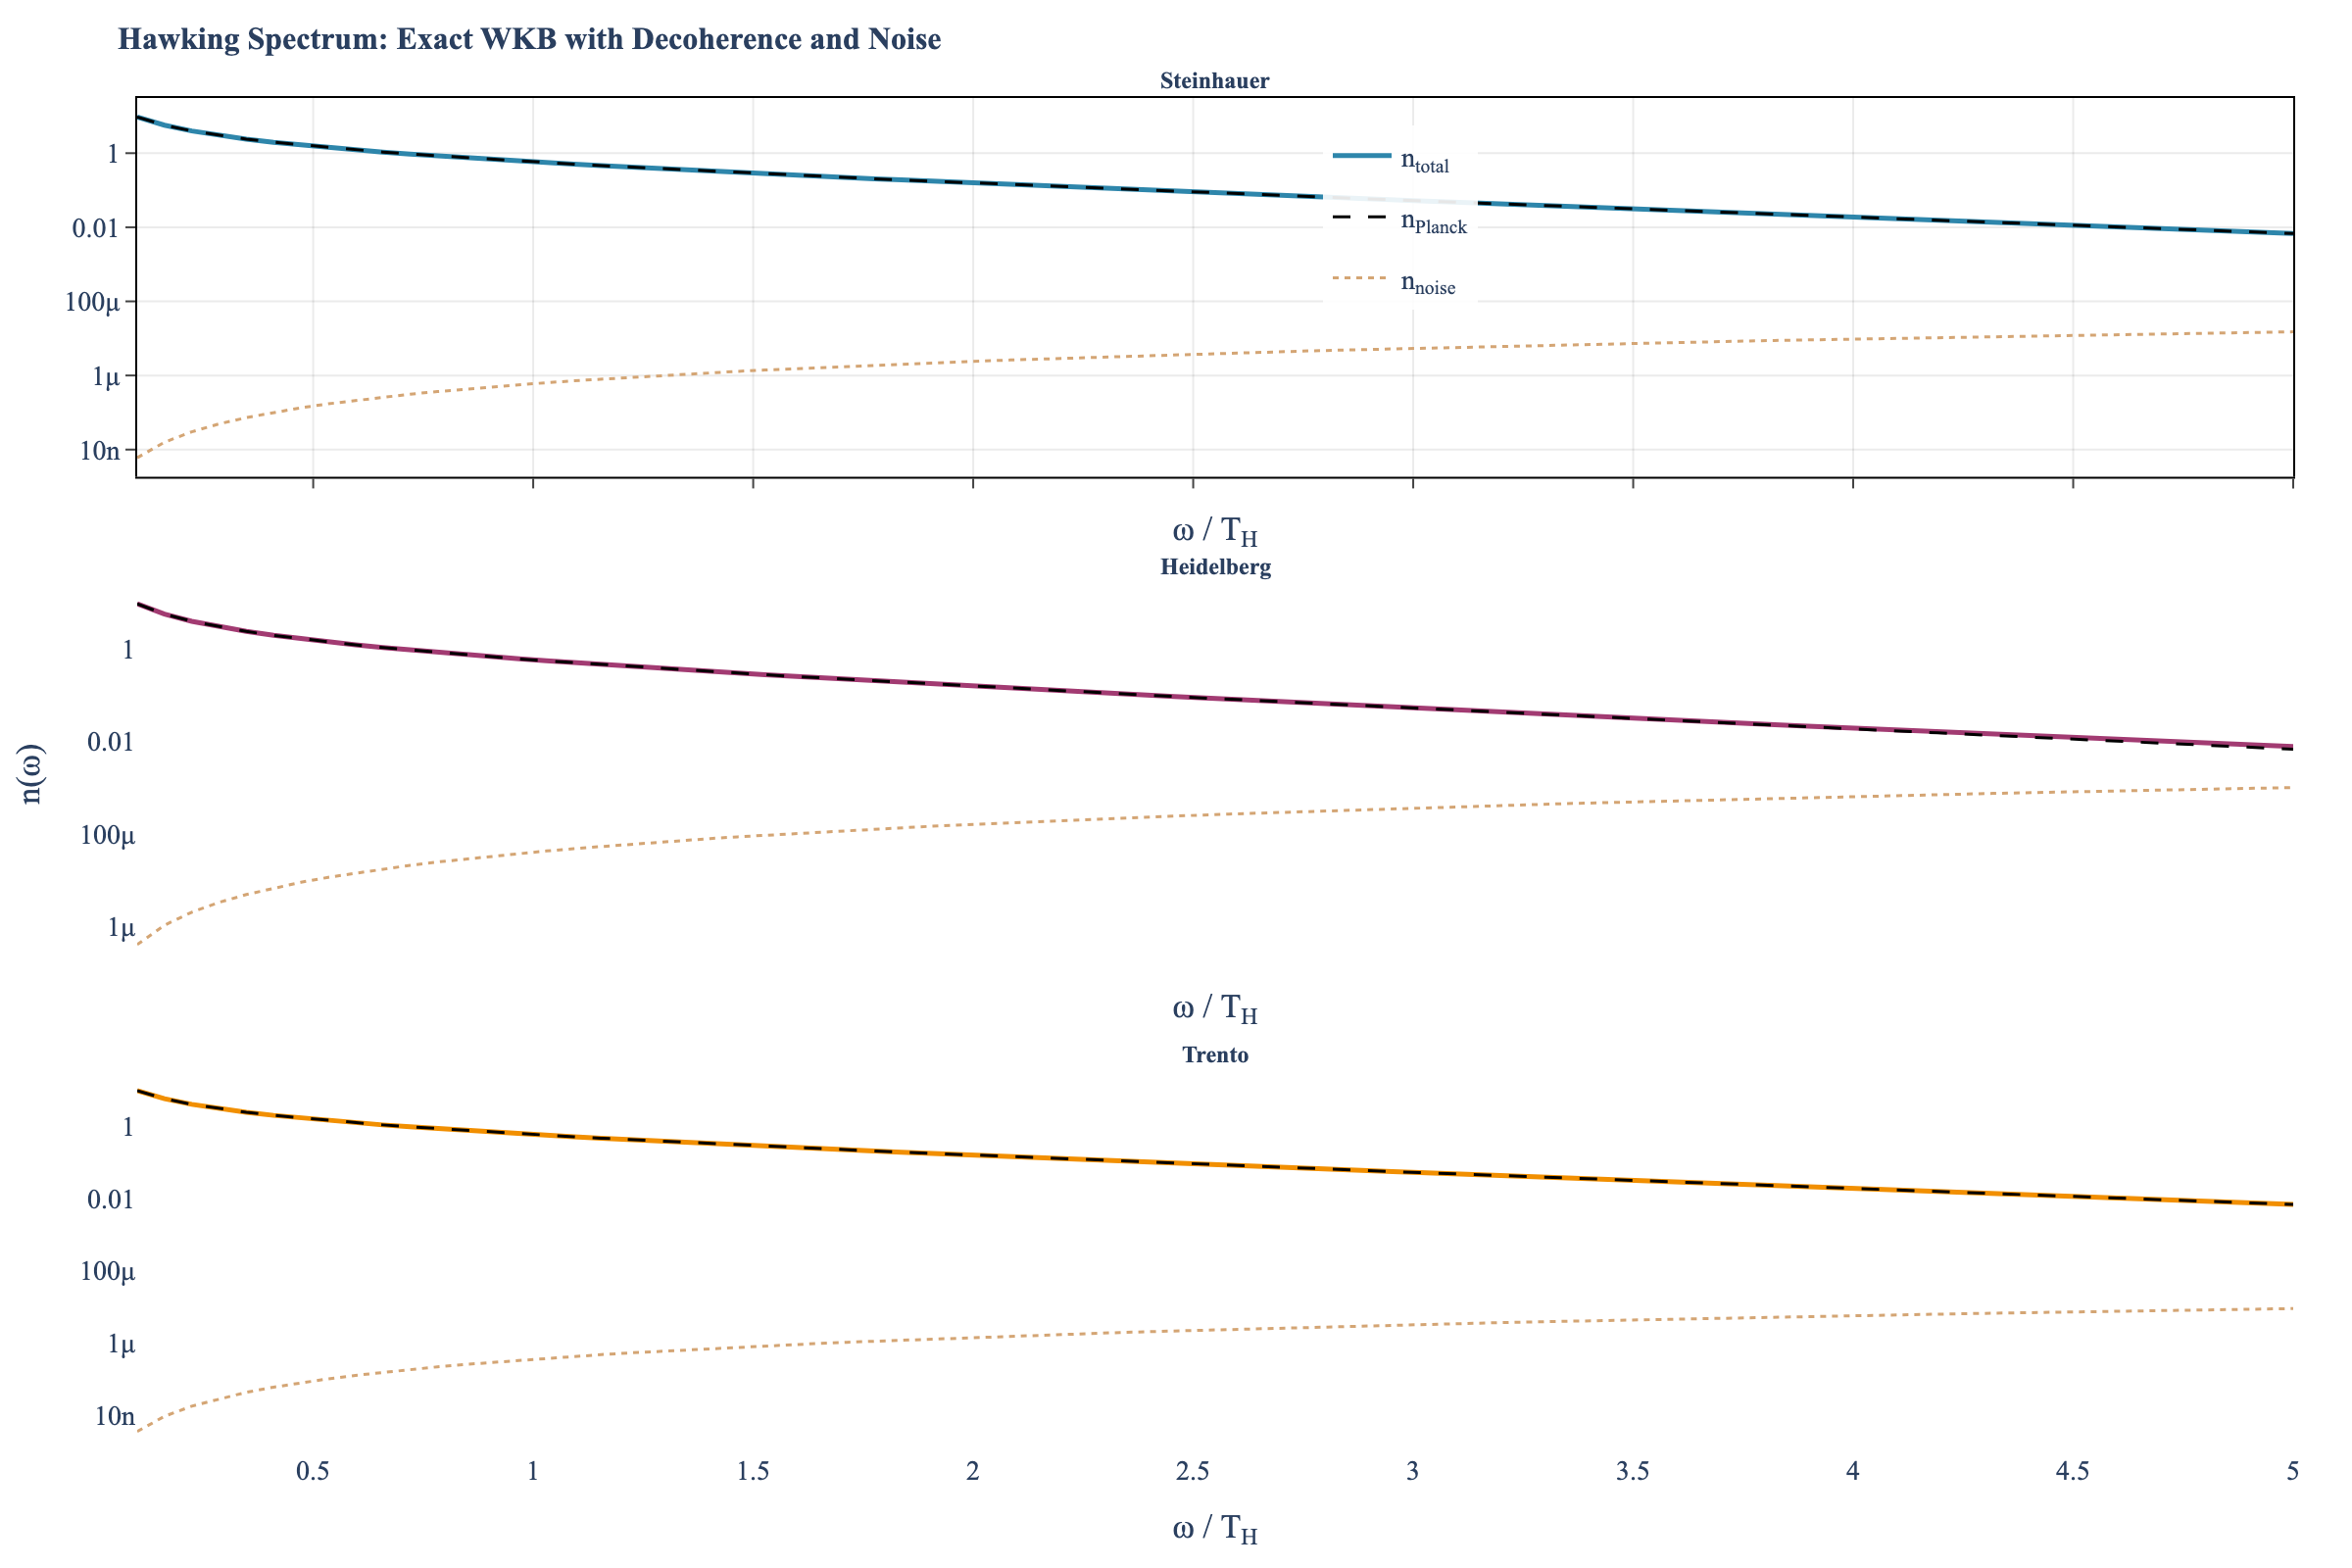
\includegraphics[width=\columnwidth]{figures/fig25_hawking_spectrum_exact.png}
\caption{Full Hawking spectrum with exact WKB corrections for three BEC
platforms. Each panel shows total occupation $n(\omega)$ (solid), standard
Planck $n_\text{Planck}$ (dashed), and FDR noise floor $n_\text{noise}$
(dotted). The spectral floor where $n_\text{noise} > n_\text{Hawking}$ is
visible at high frequencies.}
\label{fig:spectrum}
\end{figure}

%═══════════════════════════════════════════════════════
\section{Platform Predictions}
%═══════════════════════════════════════════════════════

We evaluate the exact WKB formula for three BEC platforms:

\begin{table}[h]
\begin{ruledtabular}
\begin{tabular}{lccc}
 & Steinhauer & Heidelberg & Trento \\
 & ${}^{87}$Rb & ${}^{39}$K & ${}^{23}$Na \\
\hline
$D$ & 0.03 & 0.02 & 0.014 \\
$\gamma_\text{dim}$ & 0.003 & 0.002 & $1.4\times10^{-5}$ \\
$\delta_\text{diss}(T_H)$ & $7.6\times10^{-5}$ & $3.4\times10^{-5}$ & $1.7\times10^{-7}$ \\
$\delta_k(T_H)$ & $1.5\times10^{-4}$ & $6.7\times10^{-5}$ & $3.3\times10^{-7}$ \\
$n_\text{noise}(T_H)$ & $7.6\times10^{-5}$ & $3.4\times10^{-5}$ & $1.7\times10^{-7}$ \\
$\omega_\text{max}/T_H$ & 65 & 87 & 111 \\
\end{tabular}
\end{ruledtabular}
\caption{Exact WKB parameters for three BEC platforms. All quantities
in natural units ($c_s = 1$, $\kappa = 1$). $\omega_\text{max}$ is the
dispersive UV cutoff.}
\label{tab:platforms}
\end{table}

The Trento spin-sonic platform has the smallest dissipative corrections
($\gamma_\text{dim} \sim 10^{-5}$), making it the cleanest window onto
the pure Hawking signal. However, all three platforms have
$\delta_k \ll 1$, confirming the EFT is perturbatively valid.

The noise floor provides a new experimental observable: at frequencies
above $\omega_\times$, the occupation number transitions from
Planckian decay to a power-law floor $\propto \omega^2$. Detecting
this transition would constitute direct evidence for the open-system
character of the analog Hawking effect.

%═══════════════════════════════════════════════════════
\section{Formal Verification}
%═══════════════════════════════════════════════════════

All structural results are formalized in Lean~4 using the Mathlib
library. The module \texttt{WKBConnection.lean} contains 17 theorems
with zero \texttt{sorry} gaps:

\begin{itemize}
\item \texttt{decoherence\_nonneg}: $\delta_k \geq 0$
\item \texttt{decoherence\_zero\_iff}: $\delta_k = 0 \Leftrightarrow \Gamma_H = 0$
\item \texttt{modified\_unitarity}: $|\alpha|^2 - |\beta|^2 = 1 - \delta_k$
  (structural)
\item \texttt{standard\_unitarity\_recovered}: $\Gamma_H = 0 \Rightarrow
  |\alpha|^2 - |\beta|^2 = 1$
\item \texttt{noise\_floor\_nonneg}: $n_\text{noise} \geq 0$
\item \texttt{noise\_floor\_eq\_delta\_diss}: $n_\text{noise} = \delta_\text{diss}$
\item \texttt{occupation\_reduces\_to\_beta\_sq}: $\Gamma_H = 0 \Rightarrow
  n = |\beta|^2$
\item \texttt{noise\_dominates\_when\_beta\_small}: spectral floor theorem
\item \texttt{turning\_point\_shift\_pos\_iff}: $\delta x > 0 \Leftrightarrow
  \Gamma_H > 0$
\end{itemize}

Combined with the full project formalization across 30 Lean modules,
the project contains 429 theorems plus 2 axioms
(99 Aristotle-proved across 27 runs, remainder manual), all sorry-free.

\begin{figure}[htb]
\centering
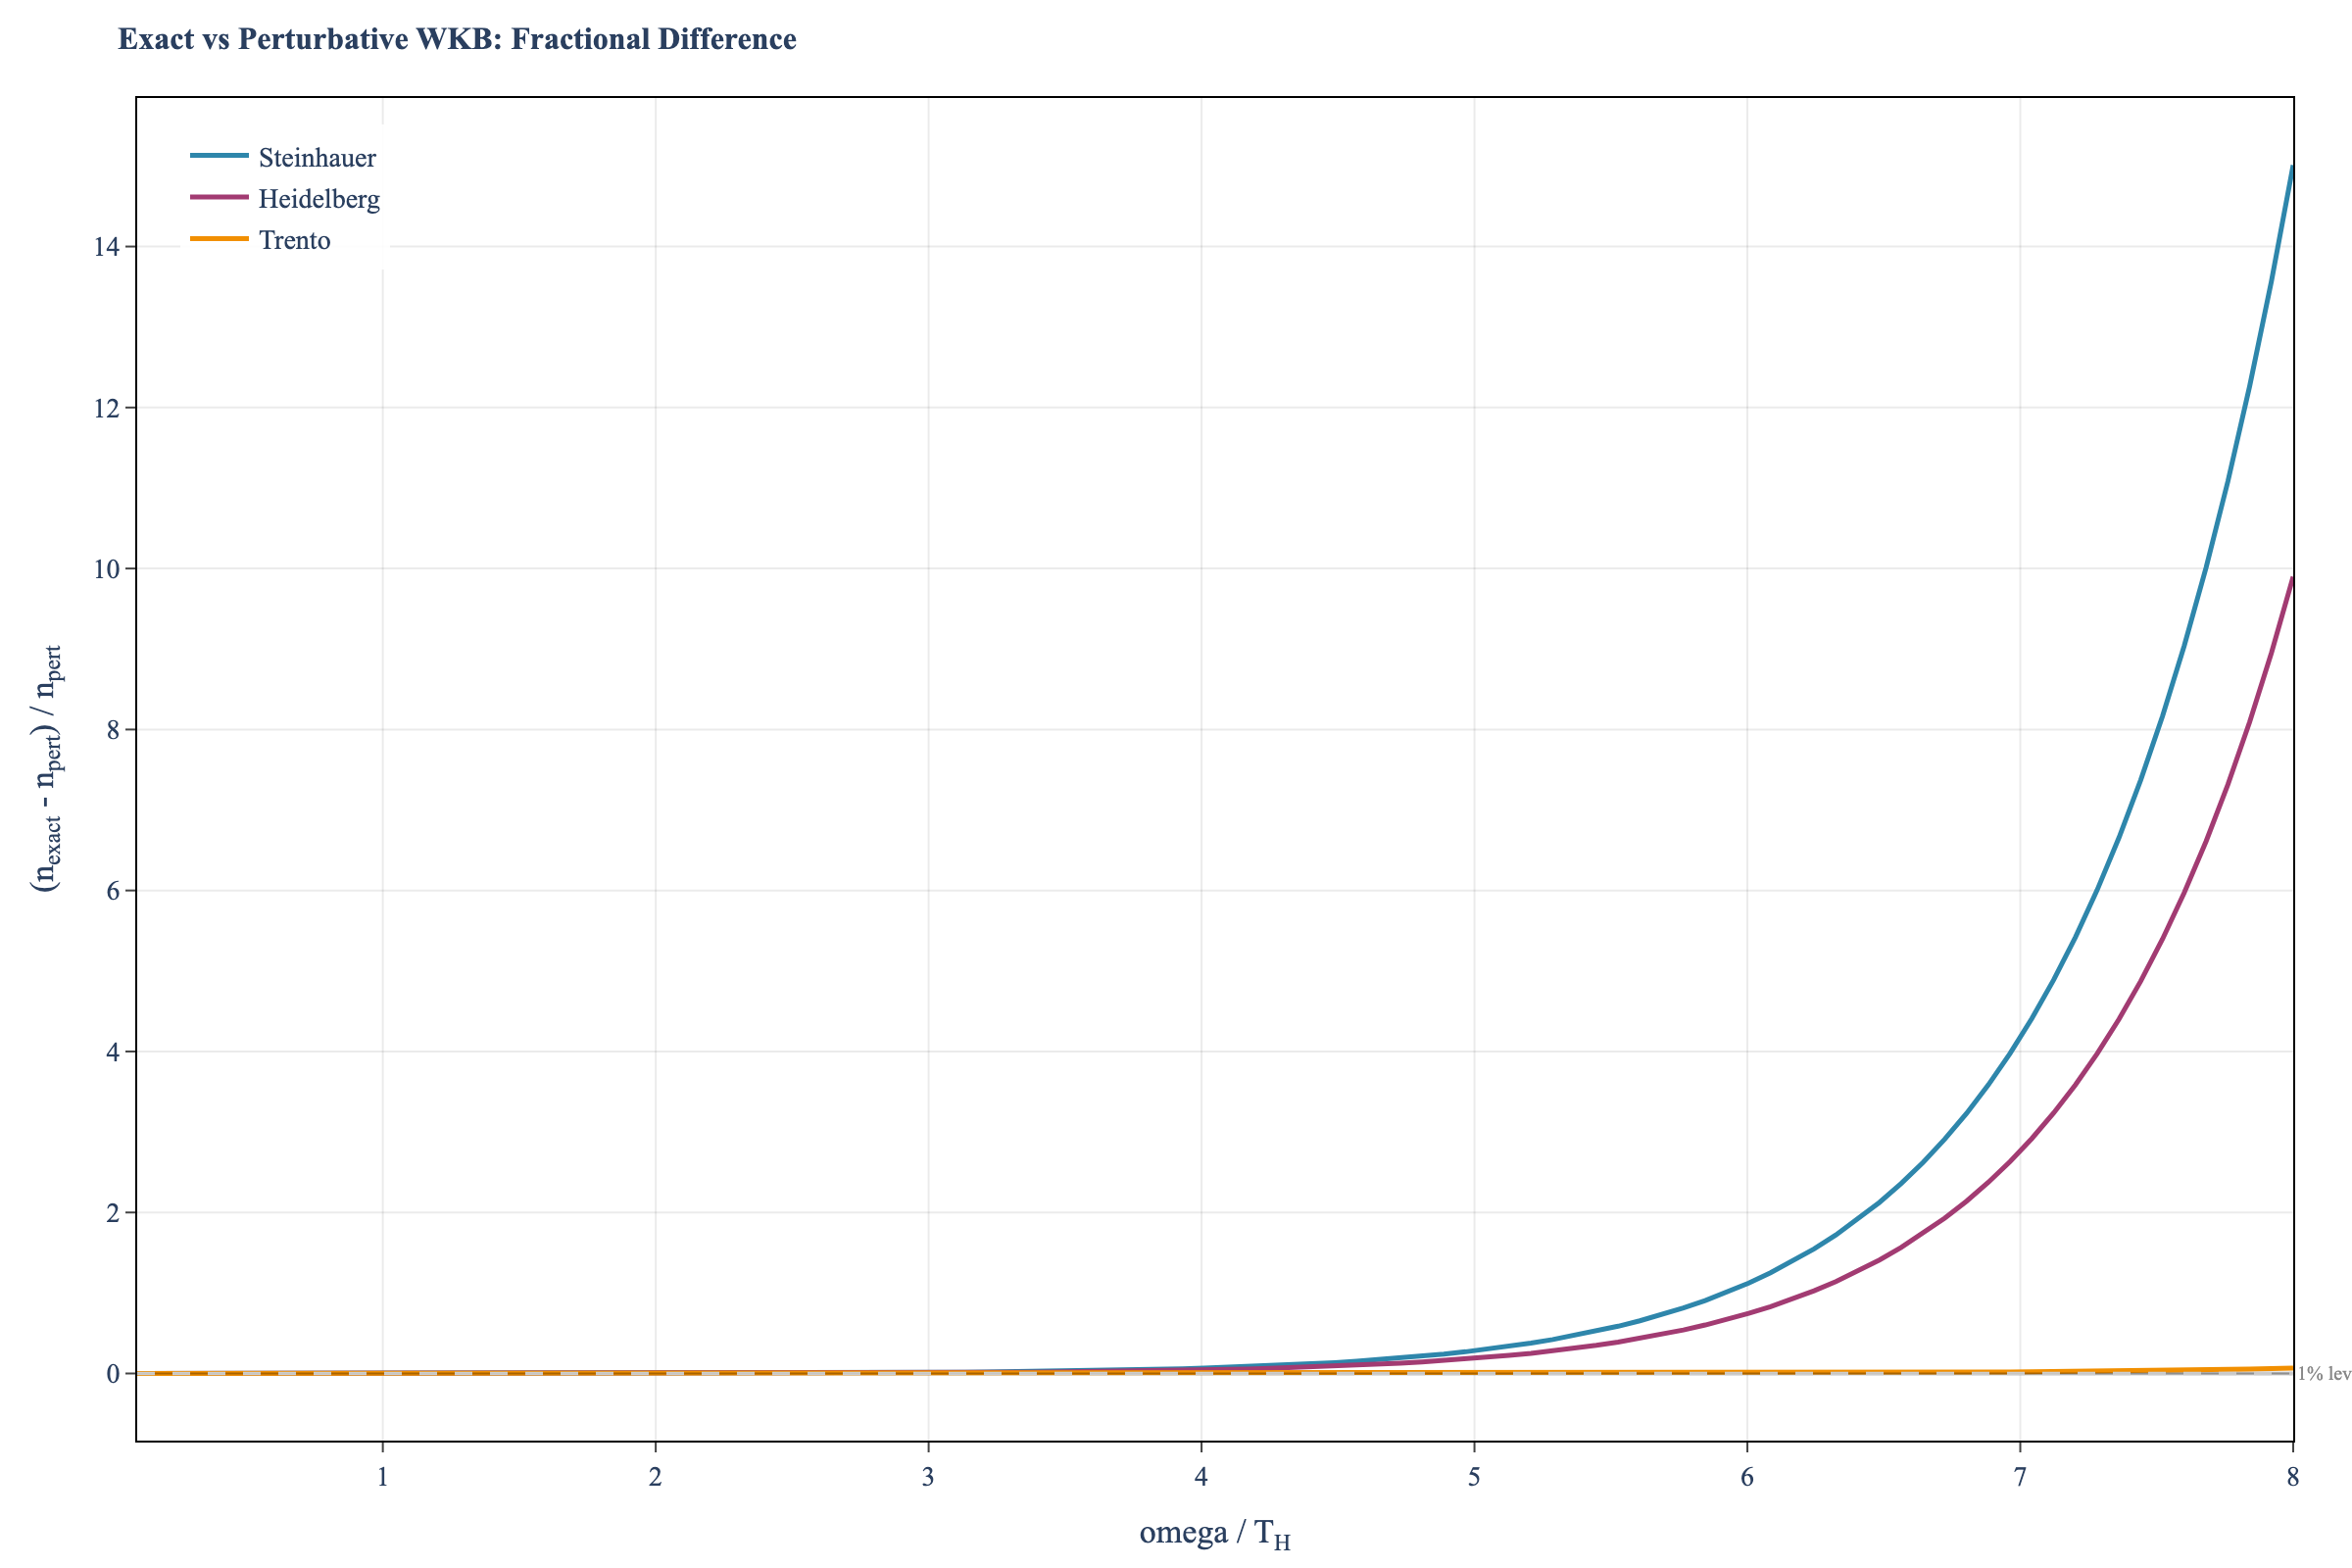
\includegraphics[width=\columnwidth]{figures/fig27_exact_vs_perturbative.png}
\caption{Fractional difference between the exact WKB occupation number
and the perturbative EFT result, $(n_\text{exact} - n_\text{pert})/n_\text{pert}$,
vs.\ frequency for three platforms. The divergence at high $\omega$ reflects
the noise floor and decoherence corrections absent from the perturbative treatment.}
\label{fig:exact_vs_pert}
\end{figure}

%═══════════════════════════════════════════════════════
\section{Discussion}
%═══════════════════════════════════════════════════════

The exact WKB connection formula reveals three non-perturbative effects
that are invisible in the perturbative EFT treatment:

\textit{Modified unitarity.} The decoherence parameter $\delta_k = 2\delta_\text{diss}$
is numerically small for current BEC experiments ($\sim 10^{-4}$), but its
existence is a qualitative statement about the open-system nature of analog
Hawking radiation. It implies that Hawking pairs are partially decohered by
the microscopic environment, with entanglement degradation $\sim \delta_k/2$.

\textit{Spectral floor.} The transition from Planckian decay to a power-law
noise floor at $\omega_\times \approx 6\,T_H$ is a sharp, qualitative
prediction. While the transition frequency depends on the specific damping
rate, its existence is universal for any dissipative analog system.

\textit{Consistency.} At leading order, the exact formula reduces to the
perturbative result: $\kappa_\text{eff} = \kappa/(1 + \delta_\text{diss})$
and $n \approx 1/(e^{2\pi\omega/\kappa_\text{eff}} - 1)$. The non-perturbative
corrections are parametrically suppressed by $\delta_\text{diss}^2$ and
only become significant at high frequencies or for strongly dissipative systems.

%═══════════════════════════════════════════════════════
\section{Conclusion}
%═══════════════════════════════════════════════════════

We have derived the exact WKB connection formula for dissipative analog
Hawking radiation, completing the theoretical chain from SK-EFT transport
coefficients to observable Hawking spectrum. The modified unitarity relation,
FDR noise floor, and spectral floor constitute three qualitatively new
predictions beyond the perturbative EFT. These results, formally verified
in Lean~4, provide the foundation for quantitative comparison with
next-generation BEC Hawking radiation experiments.

\begin{acknowledgments}
This work was conducted with the assistance of Claude Code (Anthropic).
All Lean~4 formal proofs were verified against Mathlib.
\end{acknowledgments}

\begin{thebibliography}{99}
\bibitem{Unruh1981} W.~G.~Unruh, Phys.\ Rev.\ Lett.\ \textbf{46}, 1351 (1981).
\bibitem{Steinhauer2016} J.~Steinhauer, Nat.\ Phys.\ \textbf{12}, 959 (2016).
\bibitem{deNova2019} J.~R.~M.~de~Nova, K.~Golubkov, V.~I.~Kolobov, and J.~Steinhauer, Nature \textbf{569}, 688 (2019).
\bibitem{Berry1989} M.~V.~Berry, Proc.\ R.\ Soc.\ A \textbf{422}, 7 (1989).
\bibitem{Heading1962} J.~Heading, \emph{An Introduction to Phase-Integral Methods} (Wiley, 1962).
\bibitem{CorleyJacobson1996} S.~Corley and T.~Jacobson, Phys.\ Rev.\ D \textbf{54}, 1568 (1996).
\bibitem{CoutantParentani2012} A.~Coutant, R.~Parentani, and S.~Finazzi, Phys.\ Rev.\ D \textbf{85}, 024021 (2012).
\bibitem{BelgiornoCacciatori2024} F.~Belgiorno, S.~L.~Cacciatori, and D.~Trevisan, Universe \textbf{10}, 412 (2024).
\bibitem{RobertsonParentani2015} S.~Robertson and R.~Parentani, Phys.\ Rev.\ D \textbf{92}, 044043 (2015).
\bibitem{LombardoTuriaci2012} F.~C.~Lombardo and G.~J.~Turiaci, Phys.\ Rev.\ Lett.\ \textbf{108}, 261301 (2012).
\bibitem{JanaLoganayagam2020} S.~Jana, R.~Loganayagam, and M.~Rangamani, JHEP \textbf{2020} (2020).
\bibitem{GiacobinoJacquet2025} A.~Giacobino and M.~J.~Jacquet, arXiv:2512.14194 (2025).
\end{thebibliography}

\end{document}
